\begin{minipage}{0.75\linewidth}
\begin{figure}[h]
    \centering
    \begin{adjustbox}{max width=1.0\linewidth, keepaspectratio}
        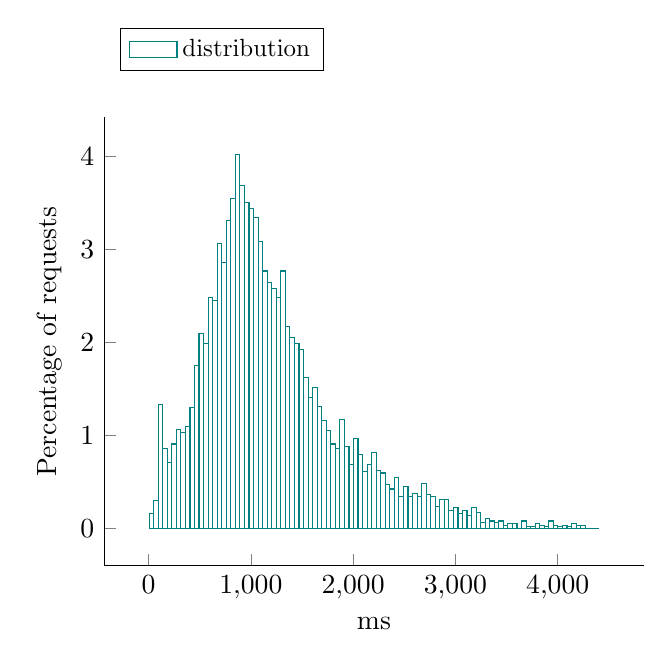
\begin{tikzpicture}
            \begin{axis}[ylabel = Percentage of requests, 
xlabel = ms, 
legend style = {nodes={scale=0.9, transform shape}, at={(0.03,1.2)}, anchor=north west, draw=black, fill=white, align=left, legend columns=3},
area style, mark size = 0pt,
 cycle list name = exotic,
  axis lines* = left]
		\addplot +[ybar interval] coordinates {
			 (5, 0.15625)
			 (49.41, 0.296875)
			 (93.82, 1.32812)
			 (138.23, 0.859375)
			 (182.64, 0.703125)
			 (227.05, 0.90625)
			 (271.46, 1.0625)
			 (315.87, 1.03125)
			 (360.28, 1.09375)
			 (404.69, 1.29688)
			 (449.1, 1.75)
			 (493.51, 2.09375)
			 (537.92, 1.98438)
			 (582.33, 2.48438)
			 (626.74, 2.45312)
			 (671.15, 3.0625)
			 (715.56, 2.85938)
			 (759.97, 3.3125)
			 (804.38, 3.54688)
			 (848.79, 4.01562)
			 (893.2, 3.6875)
			 (937.61, 3.5)
			 (982.02, 3.4375)
			 (1026.43, 3.34375)
			 (1070.84, 3.07812)
			 (1115.25, 2.76562)
			 (1159.66, 2.64062)
			 (1204.07, 2.57812)
			 (1248.48, 2.48438)
			 (1292.89, 2.76562)
			 (1337.3, 2.17188)
			 (1381.71, 2.04688)
			 (1426.12, 1.98438)
			 (1470.53, 1.92188)
			 (1514.94, 1.625)
			 (1559.35, 1.40625)
			 (1603.76, 1.51562)
			 (1648.17, 1.3125)
			 (1692.58, 1.15625)
			 (1736.99, 1.04688)
			 (1781.4, 0.90625)
			 (1825.81, 0.859375)
			 (1870.22, 1.17188)
			 (1914.63, 0.875)
			 (1959.04, 0.6875)
			 (2003.45, 0.96875)
			 (2047.86, 0.796875)
			 (2092.27, 0.609375)
			 (2136.68, 0.6875)
			 (2181.09, 0.8125)
			 (2225.5, 0.625)
			 (2269.91, 0.59375)
			 (2314.32, 0.46875)
			 (2358.73, 0.421875)
			 (2403.14, 0.546875)
			 (2447.55, 0.34375)
			 (2491.96, 0.453125)
			 (2536.37, 0.34375)
			 (2580.78, 0.375)
			 (2625.19, 0.34375)
			 (2669.6, 0.484375)
			 (2714.01, 0.359375)
			 (2758.42, 0.34375)
			 (2802.83, 0.234375)
			 (2847.24, 0.3125)
			 (2891.65, 0.3125)
			 (2936.06, 0.1875)
			 (2980.47, 0.21875)
			 (3024.88, 0.15625)
			 (3069.29, 0.1875)
			 (3113.7, 0.140625)
			 (3158.11, 0.21875)
			 (3202.52, 0.171875)
			 (3246.93, 0.0625)
			 (3291.34, 0.109375)
			 (3335.75, 0.078125)
			 (3380.16, 0.0625)
			 (3424.57, 0.078125)
			 (3468.98, 0.03125)
			 (3513.39, 0.046875)
			 (3557.8, 0.046875)
			 (3602.21, 0)
			 (3646.62, 0.078125)
			 (3691.03, 0.015625)
			 (3735.44, 0.015625)
			 (3779.85, 0.046875)
			 (3824.26, 0.03125)
			 (3868.67, 0.015625)
			 (3913.08, 0.078125)
			 (3957.49, 0.03125)
			 (4001.9, 0.015625)
			 (4046.31, 0.03125)
			 (4090.72, 0.015625)
			 (4135.13, 0.046875)
			 (4179.54, 0.03125)
			 (4223.95, 0.03125)
			 (4268.36, 0)
			 (4312.77, 0)
			 (4357.18, 0)
			 (4401.59, 0)
		};
\addlegendentry{distribution};
           \end{axis}
      \end{tikzpicture}
  \end{adjustbox}
  \caption{Response time distribution - req = ReadTimeline-2}
\end{figure}
\end{minipage}\hfill\begin{minipage}{0.18\linewidth}
\begin{table}[h]
\begin{tabular}{|cc|}
\hline
\textbf{} & \textbf{ms}\\ \hline
 \Xhline{0.005\arrayrulewidth}
min & 5\\
 \Xhline{0.005\arrayrulewidth}
max & 4446\\
 \Xhline{0.005\arrayrulewidth}
mean & 1207\\
 \Xhline{0.005\arrayrulewidth}
std & 679\\
\hline
\hline
 \Xhline{0.005\arrayrulewidth}
25th & 753\\
 \Xhline{0.005\arrayrulewidth}
50th & 1064\\
 \Xhline{0.005\arrayrulewidth}
75th & 1523\\
 \Xhline{0.005\arrayrulewidth}
80th & 1673\\
 \Xhline{0.005\arrayrulewidth}
85th & 1889\\
 \Xhline{0.005\arrayrulewidth}
90th & 2163\\
 \Xhline{0.005\arrayrulewidth}
95th & 2596\\
 \Xhline{0.005\arrayrulewidth}
99th & 3263\\
\hline
\end{tabular}
\caption{Response time}
\end{table}
\end{minipage}\hfill